\PassOptionsToPackage{unicode=true}{hyperref} % options for packages loaded elsewhere
\PassOptionsToPackage{hyphens}{url}
%
\documentclass[english,man]{apa6}
\usepackage{lmodern}
\usepackage{amssymb,amsmath}
\usepackage{ifxetex,ifluatex}
\usepackage{fixltx2e} % provides \textsubscript
\ifnum 0\ifxetex 1\fi\ifluatex 1\fi=0 % if pdftex
  \usepackage[T1]{fontenc}
  \usepackage[utf8]{inputenc}
  \usepackage{textcomp} % provides euro and other symbols
\else % if luatex or xelatex
  \usepackage{unicode-math}
  \defaultfontfeatures{Ligatures=TeX,Scale=MatchLowercase}
\fi
% use upquote if available, for straight quotes in verbatim environments
\IfFileExists{upquote.sty}{\usepackage{upquote}}{}
% use microtype if available
\IfFileExists{microtype.sty}{%
\usepackage[]{microtype}
\UseMicrotypeSet[protrusion]{basicmath} % disable protrusion for tt fonts
}{}
\IfFileExists{parskip.sty}{%
\usepackage{parskip}
}{% else
\setlength{\parindent}{0pt}
\setlength{\parskip}{6pt plus 2pt minus 1pt}
}
\usepackage{hyperref}
\hypersetup{
            pdftitle={Writing an academic paper using papaja and RStudio: A moderated mediation diary study},
            pdfkeywords={motivation, cognition, zombies, pancakes},
            pdfborder={0 0 0},
            breaklinks=true}
\urlstyle{same}  % don't use monospace font for urls
\usepackage{graphicx,grffile}
\makeatletter
\def\maxwidth{\ifdim\Gin@nat@width>\linewidth\linewidth\else\Gin@nat@width\fi}
\def\maxheight{\ifdim\Gin@nat@height>\textheight\textheight\else\Gin@nat@height\fi}
\makeatother
% Scale images if necessary, so that they will not overflow the page
% margins by default, and it is still possible to overwrite the defaults
% using explicit options in \includegraphics[width, height, ...]{}
\setkeys{Gin}{width=\maxwidth,height=\maxheight,keepaspectratio}
\setlength{\emergencystretch}{3em}  % prevent overfull lines
\providecommand{\tightlist}{%
  \setlength{\itemsep}{0pt}\setlength{\parskip}{0pt}}
\setcounter{secnumdepth}{0}

% set default figure placement to htbp
\makeatletter
\def\fps@figure{htbp}
\makeatother

% Manuscript styling
\usepackage{upgreek}
\captionsetup{font=singlespacing,justification=justified}

% Table formatting
\usepackage{longtable}
\usepackage{lscape}
% \usepackage[counterclockwise]{rotating}   % Landscape page setup for large tables
\usepackage{multirow}		% Table styling
\usepackage{tabularx}		% Control Column width
\usepackage[flushleft]{threeparttable}	% Allows for three part tables with a specified notes section
\usepackage{threeparttablex}            % Lets threeparttable work with longtable

% Create new environments so endfloat can handle them
% \newenvironment{ltable}
%   {\begin{landscape}\begin{center}\begin{threeparttable}}
%   {\end{threeparttable}\end{center}\end{landscape}}
\newenvironment{lltable}{\begin{landscape}\begin{center}\begin{ThreePartTable}}{\end{ThreePartTable}\end{center}\end{landscape}}

% Enables adjusting longtable caption width to table width
% Solution found at http://golatex.de/longtable-mit-caption-so-breit-wie-die-tabelle-t15767.html
\makeatletter
\newcommand\LastLTentrywidth{1em}
\newlength\longtablewidth
\setlength{\longtablewidth}{1in}
\newcommand{\getlongtablewidth}{\begingroup \ifcsname LT@\roman{LT@tables}\endcsname \global\longtablewidth=0pt \renewcommand{\LT@entry}[2]{\global\advance\longtablewidth by ##2\relax\gdef\LastLTentrywidth{##2}}\@nameuse{LT@\roman{LT@tables}} \fi \endgroup}

% \setlength{\parindent}{0.5in}
% \setlength{\parskip}{0pt plus 0pt minus 0pt}

% \usepackage{etoolbox}
\makeatletter
\patchcmd{\HyOrg@maketitle}
  {\section{\normalfont\normalsize\abstractname}}
  {\section*{\normalfont\normalsize\abstractname}}
  {}{\typeout{Failed to patch abstract.}}
\makeatother
\shorttitle{writing with papaja}
\author{Henrik Sørlie\textsuperscript{1,2,3}, Mads Medforfatter\textsuperscript{2,3}, \& Pernille Psykolog\textsuperscript{1,3}}
\affiliation{
\vspace{0.5cm}
\textsuperscript{1} Norwegian Defence Command and Staff College, Norwegian Defence University College\\\textsuperscript{2} Department of Psychosocial Science, University of Bergen\\\textsuperscript{3} Institutt for kvasipsykologi, Livets Harde Høgskole}
\authornote{
The authors declare no conflict of interest.


Correspondence concerning this article should be addressed to Henrik Sørlie, Artikkelgata 1, 0001 Oslo. E-mail: henrik.sorlie@uib.no}
\keywords{motivation, cognition, zombies, pancakes\newline\indent Word count: 1356}
\DeclareDelayedFloatFlavor{ThreePartTable}{table}
\DeclareDelayedFloatFlavor{lltable}{table}
\DeclareDelayedFloatFlavor*{longtable}{table}
\makeatletter
\renewcommand{\efloat@iwrite}[1]{\immediate\expandafter\protected@write\csname efloat@post#1\endcsname{}}
\makeatother
\usepackage{lineno}

\linenumbers
\usepackage{csquotes}
\ifnum 0\ifxetex 1\fi\ifluatex 1\fi=0 % if pdftex
  \usepackage[shorthands=off,main=english]{babel}
\else
  % load polyglossia as late as possible as it *could* call bidi if RTL lang (e.g. Hebrew or Arabic)
  \usepackage{polyglossia}
  \setmainlanguage[]{english}
\fi

\title{Writing an academic paper using papaja and RStudio: A moderated mediation diary study}

\date{}

\abstract{
One or two sentences providing a \textbf{basic introduction} to the field, comprehensible to a scientist in any discipline.

Two to three sentences of \textbf{more detailed background}, comprehensible to scientists in related disciplines.

One sentence clearly stating the \textbf{general problem} being addressed by this particular study.

One sentence summarizing the main result (with the words ``\textbf{here we show}'' or their equivalent).

Two or three sentences explaining what the \textbf{main result} reveals in direct comparison to what was thought to be the case previously, or how the main result adds to previous knowledge.

One or two sentences to put the results into a more \textbf{general context}.

Two or three sentences to provide a \textbf{broader perspective}, readily comprehensible to a scientist in any discipline.
}

\begin{document}
\maketitle

Life is hard.
And so is writing the introduction to a paper.
Here I have quoted some sources (Alfes, Shantz, \& Alahakone, 2016; Barrick \& Parks-Leduc, 2019).
And here I have quoted even more (Gurbuz, 2009; Koopman et al., 2019; Robison \& Unsworth, 2018).
It should be clear by now that this is a really good paper.
Thus, we hypothesize:

H1: This is an awesome paper.

\hypertarget{i-like-pancakes}{%
\section{I like pancakes}\label{i-like-pancakes}}

Pancakes are good (Deci, Olafsen, \& Ryan, 2017; Demerouti, Bakker, \& Halbesleben, 2015).
I could eat pancakes all day.

H2: This hypothesis is better than the last one.

\hypertarget{methods}{%
\section{Methods}\label{methods}}

\hypertarget{participants}{%
\subsection{Participants}\label{participants}}

Our sample consisted of 100 first-year psychology students, of which sixty-six were female and thirty-four were male.
The mean age was 23.69 years (\(SD = 4.71\)).

\hypertarget{material}{%
\subsection{Material}\label{material}}

\hypertarget{procedure}{%
\subsection{Procedure}\label{procedure}}

\hypertarget{data-analysis}{%
\subsection{Data analysis}\label{data-analysis}}

We used R (Version 3.6.2; R Core Team, 2019) and the R-packages \emph{dplyr} (Version 0.8.3; Wickham et al., 2019), \emph{forcats} (Version 0.4.0; Wickham, 2019a), \emph{ggplot2} (Version 3.2.1; Wickham, 2016), \emph{papaja} (Version 0.1.0.9942; Aust \& Barth, 2020), \emph{psych} (Version 1.8.12; Revelle, 2018), \emph{purrr} (Version 0.3.3; Henry \& Wickham, 2019), \emph{readr} (Version 1.3.1; Wickham, Hester, \& Francois, 2018), \emph{stringr} (Version 1.4.0; Wickham, 2019b), \emph{tibble} (Version 2.1.3; Müller \& Wickham, 2019), \emph{tidyr} (Version 1.0.2; Wickham \& Henry, 2020), and \emph{tidyverse} (Version 1.2.1; Wickham, 2017) for all our analyses.

\hypertarget{results}{%
\section{Results}\label{results}}

\begin{table}[tbp]

\begin{center}
\begin{threeparttable}

\caption{\label{tab:descriptivestable}Descriptive statistics of study variables}

\begin{tabular}{llllll}
\toprule
 & \multicolumn{1}{c}{$M$} & \multicolumn{1}{c}{$SD$} & \multicolumn{1}{c}{1} & \multicolumn{1}{c}{2} & \multicolumn{1}{c}{3}\\
\midrule
1 - Age & 23.69 & 4.71 &  &  & \\
2 - Motivation & -0.11 & 1.00 & -.10 &  & \\
3 - Pancake liking & 0.00 & 0.92 & .12 & -.08 & \\
4 - Zombieness & -0.06 & 0.63 & -.23* & .42** & .49**\\
\bottomrule
\addlinespace
\end{tabular}

\begin{tablenotes}[para]
\normalsize{\textit{Note.} * p < .05, ** p < .01, *** p < .001}
\end{tablenotes}

\end{threeparttable}
\end{center}

\end{table}

Table \ref{tab:descriptivestable} shows the means, standard deviations and correlations between all study variables. A significant correlation was found between pancakeliking and zombieness (\texttt{r}).

\hypertarget{discussion}{%
\section{Discussion}\label{discussion}}

\begin{figure}

{\centering 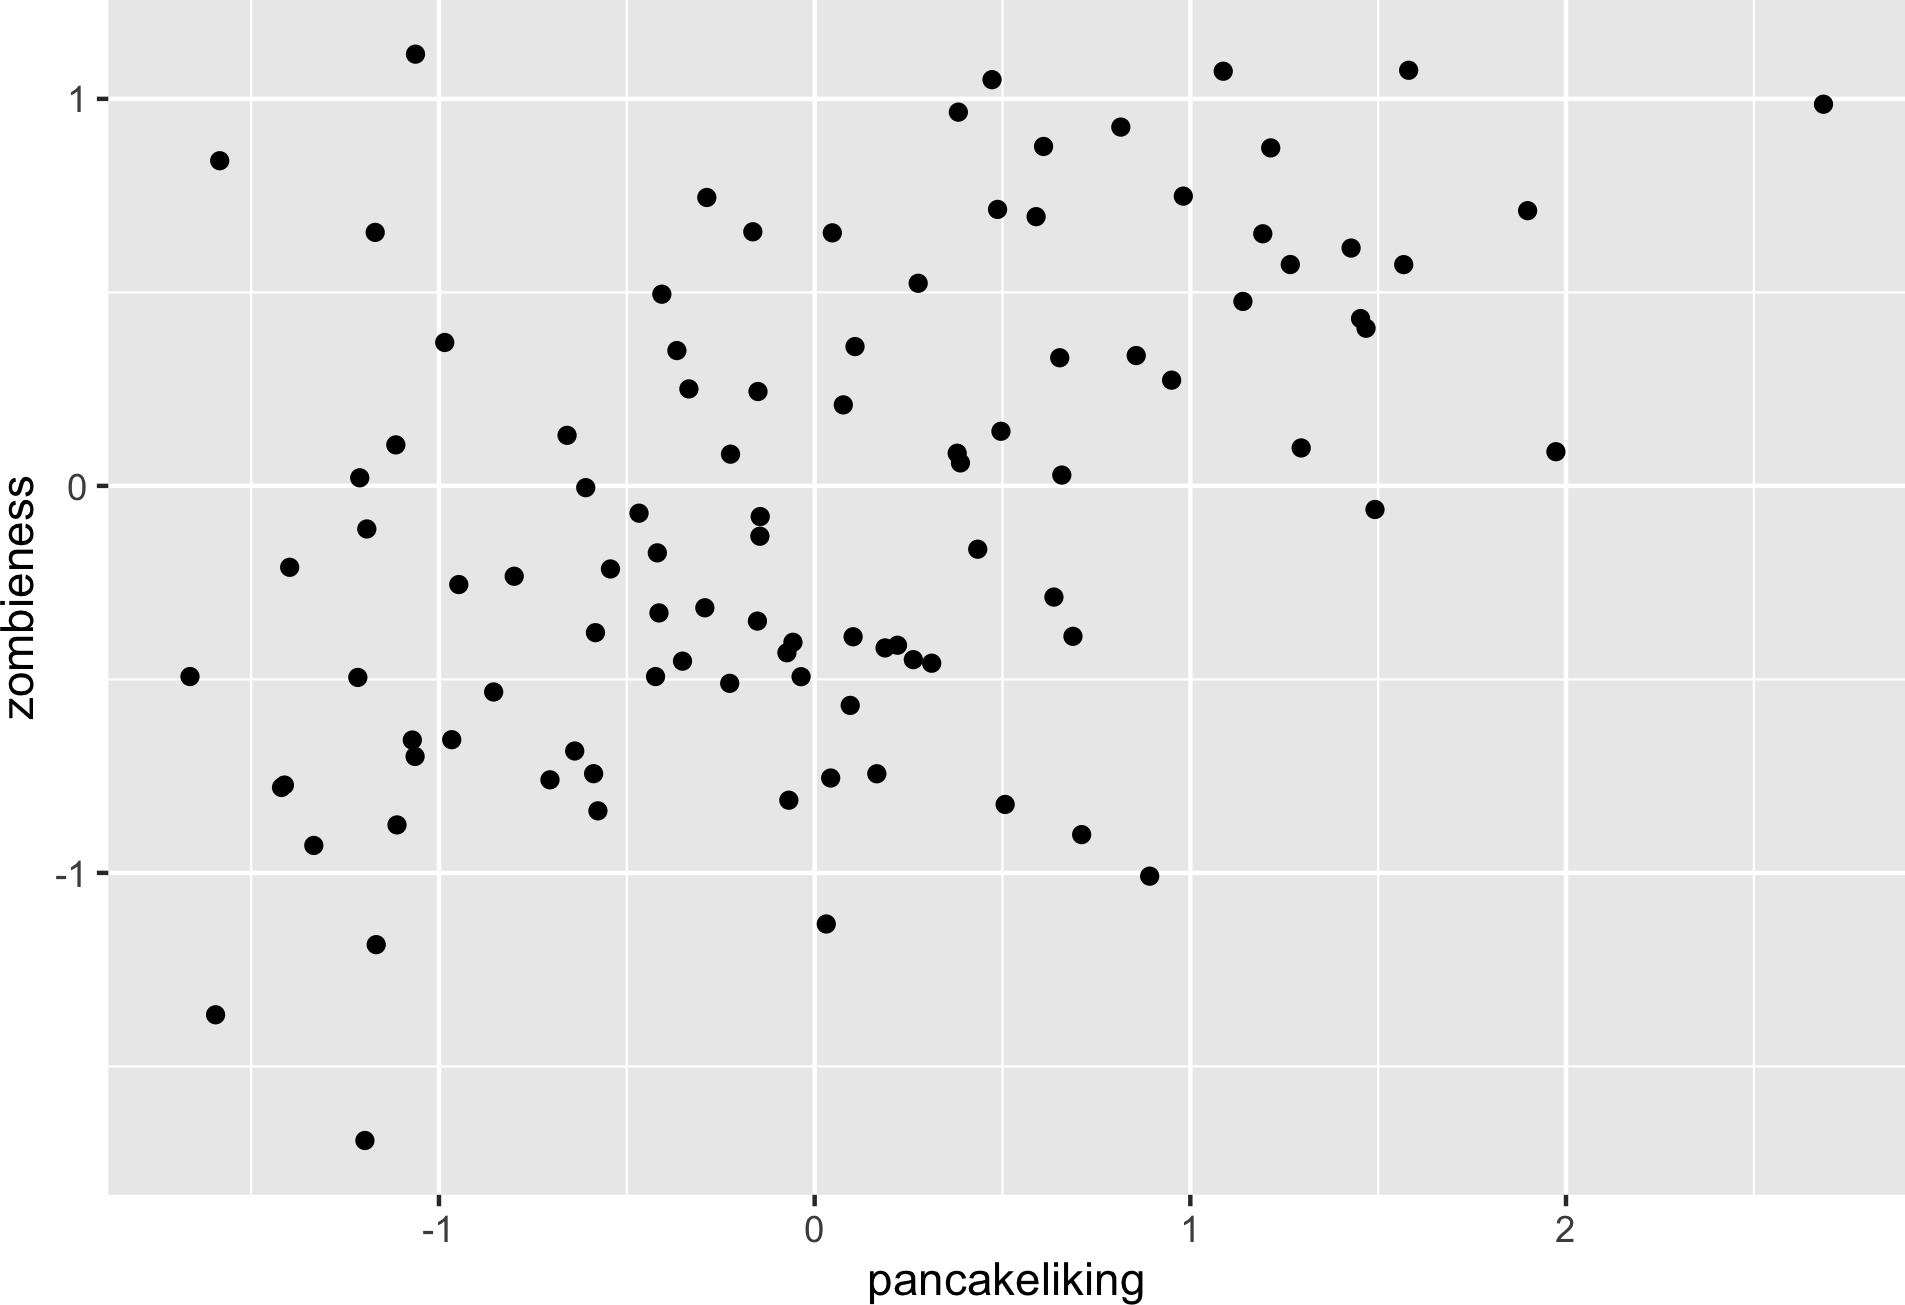
\includegraphics{testpaper_files/figure-latex/firstplot-1} 

}

\caption{This plot says it all}\label{fig:firstplot}
\end{figure}

Without a doubt, there is a lot to discuss.
As shown in figure~\ref{fig:firstplot}, our findings indicate several things.

\newpage

\hypertarget{references}{%
\section{References}\label{references}}

\begingroup
\setlength{\parindent}{-0.5in}
\setlength{\leftskip}{0.5in}

\hypertarget{refs}{}
\leavevmode\hypertarget{ref-alfesTestingAdditiveInteractive2016}{}%
Alfes, K., Shantz, A., \& Alahakone, R. (2016). Testing additive versus interactive effects of person-organization fit and organizational trust on engagement and performance. \emph{Personnel Review}, \emph{45}(6), 1323--1339. \url{https://doi.org/10.1108/PR-02-2015-0029}

\leavevmode\hypertarget{ref-R-papaja}{}%
Aust, F., \& Barth, M. (2020). \emph{papaja: Create APA manuscripts with R Markdown}. Retrieved from \url{https://github.com/crsh/papaja}

\leavevmode\hypertarget{ref-barrickSelectionFit2019a}{}%
Barrick, M. R., \& Parks-Leduc, L. (2019). Selection for Fit. \emph{Annual Review of Organizational Psychology and Organizational Behavior}, \emph{6}(1), 171--193. \url{https://doi.org/10.1146/annurev-orgpsych-012218-015028}

\leavevmode\hypertarget{ref-deciSelfDeterminationTheoryWork2017}{}%
Deci, E. L., Olafsen, A. H., \& Ryan, R. M. (2017). Self-Determination Theory in Work Organizations: The State of a Science. \emph{Annual Review of Organizational Psychology and Organizational Behavior}, \emph{4}(1), 19--43. \url{https://doi.org/10.1146/annurev-orgpsych-032516-113108}

\leavevmode\hypertarget{ref-demeroutiProductiveCounterproductiveJob2015}{}%
Demerouti, E., Bakker, A. B., \& Halbesleben, J. R. B. (2015). Productive and counterproductive job crafting: A daily diary study. \emph{Journal of Occupational Health Psychology}, \emph{20}(4), 457--469. \url{https://doi.org/10.1037/a0039002}

\leavevmode\hypertarget{ref-gurbuzPossibleAntecedentsMilitary2009a}{}%
Gurbuz, S. (2009). Some Possible Antecedents of Military Personnel Organizational Citizenship Behavior. \emph{Military Psychology}, \emph{21}(2), 200--215. \url{https://doi.org/10.1080/08995600802574621}

\leavevmode\hypertarget{ref-R-purrr}{}%
Henry, L., \& Wickham, H. (2019). \emph{Purrr: Functional programming tools}. Retrieved from \url{https://CRAN.R-project.org/package=purrr}

\leavevmode\hypertarget{ref-koopmanWhyWhomDoes2019}{}%
Koopman, J., Rosen, C. C., Gabriel, A. S., Puranik, H., Johnson, R. E., \& Ferris, D. L. (2019). Why and for whom does the pressure to help hurt others? Affective and cognitive mechanisms linking helping pressure to workplace deviance. \emph{Personnel Psychology}, peps.12354. \url{https://doi.org/10.1111/peps.12354}

\leavevmode\hypertarget{ref-R-tibble}{}%
Müller, K., \& Wickham, H. (2019). \emph{Tibble: Simple data frames}. Retrieved from \url{https://CRAN.R-project.org/package=tibble}

\leavevmode\hypertarget{ref-R-base}{}%
R Core Team. (2019). \emph{R: A language and environment for statistical computing}. Vienna, Austria: R Foundation for Statistical Computing. Retrieved from \url{https://www.R-project.org/}

\leavevmode\hypertarget{ref-R-psych}{}%
Revelle, W. (2018). \emph{Psych: Procedures for psychological, psychometric, and personality research}. Evanston, Illinois: Northwestern University. Retrieved from \url{https://CRAN.R-project.org/package=psych}

\leavevmode\hypertarget{ref-robisonPupillometryTracksFluctuations2018}{}%
Robison, M. K., \& Unsworth, N. (2018). Pupillometry tracks fluctuations in working memory performance. \emph{PsyArXiv}. \url{https://doi.org/10/gdz63r}

\leavevmode\hypertarget{ref-R-ggplot2}{}%
Wickham, H. (2016). \emph{Ggplot2: Elegant graphics for data analysis}. Springer-Verlag New York. Retrieved from \url{https://ggplot2.tidyverse.org}

\leavevmode\hypertarget{ref-R-tidyverse}{}%
Wickham, H. (2017). \emph{Tidyverse: Easily install and load the 'tidyverse'}. Retrieved from \url{https://CRAN.R-project.org/package=tidyverse}

\leavevmode\hypertarget{ref-R-forcats}{}%
Wickham, H. (2019a). \emph{Forcats: Tools for working with categorical variables (factors)}. Retrieved from \url{https://CRAN.R-project.org/package=forcats}

\leavevmode\hypertarget{ref-R-stringr}{}%
Wickham, H. (2019b). \emph{Stringr: Simple, consistent wrappers for common string operations}. Retrieved from \url{https://CRAN.R-project.org/package=stringr}

\leavevmode\hypertarget{ref-R-dplyr}{}%
Wickham, H., François, R., Henry, L., \& Müller, K. (2019). \emph{Dplyr: A grammar of data manipulation}. Retrieved from \url{https://CRAN.R-project.org/package=dplyr}

\leavevmode\hypertarget{ref-R-tidyr}{}%
Wickham, H., \& Henry, L. (2020). \emph{Tidyr: Tidy messy data}. Retrieved from \url{https://CRAN.R-project.org/package=tidyr}

\leavevmode\hypertarget{ref-R-readr}{}%
Wickham, H., Hester, J., \& Francois, R. (2018). \emph{Readr: Read rectangular text data}. Retrieved from \url{https://CRAN.R-project.org/package=readr}

\endgroup

\end{document}
